\chapter{Introduction}
\label{chap:intro}
\section{Preface}
The dynamic nature of the sky has been known for millennia. While most early records of the variable sky relate to the motion of the Sun, the planets and the Moon, the first record of extra-solar variability can be dated to 185 AD with the discovery of a ``guest star'', or supernova \citep{2006ChJAA...6..635Z}. However, the art and oral traditions of many ancient civilisations across the world describe phenomena that are broadly consistent with stellar variability \citep{2018AuJAn..29...89H} and supernovae \citep[][and references therein]{2014JAHH...17..161H}. Our understanding of the Universe and our place in it has always been shaped by the variable sky, with early cosmological theories revolving around incremental advances in observations of the planets.

It was not until the discovery of SN 1572 that a true astronomical transient shaped our understanding of the Universe \citep{1969dnen.book.....B}. While cosmology had evolved since the time of Aristotle, his belief that the Universe beyond the planets was perfect and unchanging remained the prevailing view of the time. Naked-eye observations established that the supernova exhibited no detectable parallax or proper motion, confirming that it existed beyond the planetary sphere and hence that the stars, and the Universe, are not immutable.

Over the last few centuries, advances in telescope technology have allowed astronomers to probe the Universe. We can now perform precise observations of the most distant objects in the Universe across the entire electromagnetic spectrum, and searches in the time domain remain a vital part in answering the some of the most fundamental questions in modern astronomy. Observations of supernovae are used to measure the expansion of the Universe \citep{1998AJ....116.1009R}, searches for small brightness fluctuations in stars have found thousands of planets beyond our Solar System, and observations of Fast Radio Bursts have shed light upon the decades-old problem of missing baryonic matter \citep{2020Natur.581..391M}.

The 2015 detection of gravitational waves from the merger of two black holes \citep{2016PhRvL.116f1102A} saw the dawn of a new era in time-domain astronomy, the multi-messenger era, where astronomers probe the Universe with electromagnetic radiation, gravitational waves, neutrinos and cosmic rays\footnote{Although the field began with the detection of neutrinos from SN 1987A \citep{1987PhRvL..58.1494B,1987PhRvL..58.1490H}}. However, it was not until the first detection of a neutron star merger \citep{2017PhRvL.119p1101A} that an electromagnetic counterpart to a gravitational wave event was first detected \citep{2017ApJ...848L..12A}. In the coming decades, a number of revolutionary electromagnetic and gravitational wave facilities will come online, which will drastically expand our view of the Universe and help answer many of the outstanding questions in the field. For example, what is the underlying relation between neutron star mergers and gamma-ray bursts? Can we detect gravitational waves from sources other than compact object mergers? Can we use gravitational waves to measure the expansion of the Universe, and resolve the tension between current measurements? Answering these ``known unknowns'' will also undoubtedly lead to the discovery of ``unknown unknowns'' -- unexpected discoveries that have not been predicted by theorists.

This thesis is focused on the contribution of radio observations to the multi-messenger parameter space. In this chapter I introduce the concept of gravitational waves and the process that led to their detection (\cref{sec:gw_intro}), summarise the history of gamma-ray bursts and the science behind the afterglows they produce (\cref{sec:grb_intro}), recap the discovery of GW170817 along with my contributions to the follow-up effort (\cref{sec:gw170817_intro}) and conclude by enumerating the goals of this thesis (\cref{sec:thesis_goals}).



\section{Gravitational Waves}
\label{sec:gw_intro}
\subsection{General Relativity in the Dynamical Regime}
The General Theory of Relativity proposes that gravity is the result of spacetime curvature caused by the presence of matter or energy. This reformulation of mechanics explained the long-known deviation of the orbit of Mercury from the laws of Newton and Kepler, as well as making a number of predictions for which observational evidence has since been found including the existence of black holes \citep{1972Natur.235...37W,2019ApJ...875L...1E}, gravitational lensing \citep{1979Natur.279..381W}, the deflection of light by the Sun \citep{1920RSPTA.220..291D} and gravitational redshift \citep{1925Obs....48..337A,1954ApJ...120..316P}.

In the dynamical regime, General Relativity predicts that the curvature of space time can propagate as gravitational waves. Observationally, gravitational waves manifest as small distortions of the separation between two objects. This effect is incredibly small, with the change in separation of two objects on Earth caused by waves from an extragalactic merger typically a factor of $\sim 10^{-20}$. The most common source of gravitational waves in the Universe is likely the orbital decay of a binary system consisting of either neutron stars or black holes, although there may be other sources such as some supernovae \citep{2009CQGra..26f3001O,2019ApJ...876L...9R} or single, asymmetric, neutron stars \citep{2009ASSL..357..651P}.

The discovery of PSR B1913+16 enabled the first observational study of compact binary systems \citep{1975ApJ...195L..51H}. Continued observations spanning 14 years allowed precise determination of the orbital parameters of the binary, and showed that the orbit was decaying in a manner consistent with the emission of gravitational waves \citep{1989ApJ...345..434T}. This discovery was the first indirect detection of gravitational waves and was later awarded the 1993 Nobel Prize in Physics.

Early attempts to detect gravitational waves involved the use of `Weber bars' -- large metal cylinders which should oscillate at their resonant frequency if a gravitational wave propagated through them \citep{1960PhRv..117..306W}. While there were claims of a detection using these methods \citep[e.g.][]{1969PhRvL..22.1320W}, they were later shown to be spurious. Contemporaneously to Weber, various independent groups \citep{2016Univ....2...22C} investigated the possibility of detecting gravitational waves using Michelson interferometers \citep{1887AmJS...34..333M}. Eventually this work culminated in the building of the Laser Interferometer Gravitational-Wave Observatory \citep[LIGO;][]{2015CQGra..32g4001L} and Virgo \citep{2015CQGra..32b4001A} gravitational wave detectors and ultimately led to the detection of gravitational waves from a binary black hole merger in 2015 \citep{2016PhRvL.116f1102A}. This was the first direct detection of gravitational waves and was awarded the 2017 Nobel Prize in Physics.

\begin{figure}
    \centering
    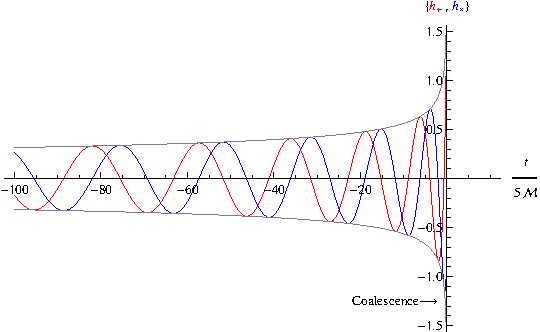
\includegraphics[trim={0cm 0cm 1cm 0cm},clip]{inspiral-waveform}
    \caption[Waveform of a compact binary coalescence inspiral]{Waveform of a compact binary coalescence inspiral, with the two gravitational wave polarisations shown in red and blue. Figure reproduced from \citet{2015PhDT.........6S}.}
    \label{fig:inspiral-waveform}
\end{figure}

\subsection{The Advanced LIGO and Virgo Detectors}
% The Advanced LIGO and Virgo detectors \citep{2015CQGra..32g4001L,2015CQGra..32b4001A} are advanced  Michelson interferometers \citep{1887AmJS...34..333M}. Each arm (3\,km for Virgo, 4\,km for both LIGO detectors) houses a Fabry-Pe\'rot cavity under ultra-high vacuum, increasing the effective length by a factor of 400. Each cavity is bookended by a silicon test mass, which is suspended on a pendulum system made of fused silica to aid in vibration isolation. Other measures to improve sensitivity include the use of power recycling mirrors to increase the effective laser power, and active vibration isolation to reduce the effects of seismic noise.

% The strain observed by a single gravitational wave interferometer produced by a compact binary coalescence consists of an oscillating signal that gradually increase in frequency and amplitude as seen in Figure \ref{fig:inspiral-waveform}. A detailed discussion of gravitational waveforms is beyond the scope of this thesis, but the signal depends not only on the intrinsic properties of the merger (the componenent spins and masses), but also extrinsic properties including the inclination angle, the distance and sky position \citep{1993PhRvD..47.2198F}.

The Advanced LIGO and Virgo detectors \citep{2015CQGra..32g4001L,2015CQGra..32b4001A} are Michelson interferometers \citep{1887AmJS...34..333M} with Fabry-Pe\'rot cavities along each arm (3\,km for Virgo, 4\,km for both LIGO detectors), that increased the effective length of the arms by a factor of 400. In the presence of gravitational waves produced by a compact binary coalescence, the distance along each arm becomes time-variable. The fractional change in distance takes the form oscillating signal that gradually increase in frequency and amplitude as seen in Figure \ref{fig:inspiral-waveform}. A detailed discussion of gravitational waveforms is beyond the scope of this thesis, but the signal depends not only on the intrinsic properties of the merger (the componenent spins and masses), but also extrinsic properties including the inclination angle, the distance and sky position \citep{1993PhRvD..47.2198F}.

\begin{figure}
    \centering
    \includesvg[width=0.7\linewidth]{mass-gap}
    \caption[Categorisation of gravitational wave events by mass]{Categorisation of compact binary coalescences during the third LIGO/Virgo observing run in terms of component masses $m_1$ and $m_2$. Four mutually exclusive astrophysical categories exist -- binary neutron stars (BNS), binary black holes (BBH), neutron star-black holes (NSBH) and ``mass gap''. Figure reproduced from the LIGO/Virgo Public Alerts User Guide (\url{https://ligo.org})}
    \label{fig:mass-gap-diagram}
\end{figure}

Signals are detected using four independent pipelines that carry out different forms of matched-filtering analysis to search for signals consistent with compact binary coalescences, while two further pipelines are used to search for unmodelled bursts like those predicted to be produced by supernovae.  Once a candidate has been detected a rapid parameter estimate is carried out using \textsc{bayestar} \citep{2016PhRvD..93b4013S}, that produces a sky-map representing the posterior probability density function of the merger's sky position. While \textsc{bayestar} computes all merger parameters, during the third observing run (O3) only limited information was publicly released prior to formal publication\footnote{\url{https://emfollow.docs.ligo.org/userguide/index.html}}. Of interest are the probabilities that at least one merger component was a neutron star, the merger produced a remnant, and the probability classification. Events are classified as either binary black hole, neutron star-black hole or binary neutron star mergers based on component masses using cutoffs of $M<3M_{\odot}$ for neutron stars and $M>5M_{\odot}$ for black holes. Any merger with at least one component in the range $3M_{\odot}<M<5M_{\odot}$ was classified as a ``mass-gap'' event (see Figure \ref{fig:mass-gap-diagram}). A final category described the probability that the event was a false-positive caused by an unrelated terrestrial signal.

Alerts are distributed via the Gamma-ray Coordinates Network\footnote{\url{https://gcn.gsfc.nasa.gov/}} (GCN) using the XML based VOEvent Transport protocol \citep{2006ASPC..351..637W}. An automated preliminary notice is distributed within minutes of a merger being detected, and is followed by a human-vetted alert approximately half an hour later. Further alerts containing updated parameter estimates are distributed in the following days. All human vetted alerts are accompanied by a GCN circular that summarises the contents of the VOEvent in human-readable form, and sometimes contains further commentary, e.g. the reason for a retraction notice. 




\section{Gamma-ray Bursts, Neutron Star Mergers \& Radio Afterglows}
\label{sec:grb_intro}
\subsection{Detection, Classification and Origins}
Recognising the detrimental effects of widespread nuclear testing, most countries signed and ratified the \textit{Treaty Banning Nuclear Weapon Tests in the Atmosphere, in Outer Space and Under Water}, which took effect in 1963. One week after the treaty was ratified, the United States launched the Vela satellites, which were capable of detecting nuclear detonations anywhere on Earth via the associated gamma-ray emission. The satellites did not detect the signature of any nuclear weapon tests, but they did detect a number of bursts of gamma-ray emission that were not consistent with a terrestrial or solar origin \citep{1973ApJ...182L..85K}. Much like gravitational waves, the existence of gamma-ray bursts was predicted prior to their discovery -- \citet{1968CaJPh..46..476C} proposed that some supernovae should produce gamma-rays as relativistic shockwaves propagate outwards through the layers of ejected material.

Twenty years after the first detections, the \textit{Burst and Transient Source Explorer} (BATSE) was launched with primary goal of detecting more bursts and discovering their origin. The large sample of bursts discovered by BATSE were distributed isotropically across the sky, suggesting an extragalactic origin \citep{1992Natur.355..143M}. It soon became clear that the distribution of burst durations is bimodal, with a divide at $\sim 2$ seconds \citep{1993ApJ...413L.101K}. The short variety makes up roughly 30\% of the population with a typical duration of 0.2\,seconds.

The large amount of energy released by the bursts combined with their non-thermal spectra suggested that they are produced by a relativistic outflow of material \citep{1975NYASA.262..164R,1986ApJ...308L..43P} that must be collimated into a jet \citep{1993NYASA.688..321P,1999ApJ...526..707P,1999ApJ...525..737R,1999ApJ...519L..17S}. A multiwavelength afterglow was predicted \citep{1993ApJ...418L...5P}, but follow-up observations were hindered by the localisation capability of BATSE, which detected bursts with positional uncertainties of $\sim 10\,\deg^2$. This was soon remedied by the launch of BeppoSAX \citep{1997A&AS..122..299B}, which contained a GRB monitor and multiple X-ray telescopes capable of localising X-ray sources with arcminute precision. Soon after launch, BeppoSAX detected a simultaneous burst of X-rays and gamma-rays \citep{1997Natur.387..783C}. Targeted follow-up observations 8 hours later revealed a fading X-ray afterglow that declined over the following few days.

While various origins for GRBs had been proposed, it was not until the detection of GRB980425 and the subsequent detection of SN1998bw, that the origin of long GRBs as core collapse supernovae was first demonstrated observationally \citep[][and references therein]{2012grb..book..169H}. The precise localisation of this burst allowed for detailed follow-up observations and confirmed the extragalactic origin of long GRBs \citep{1998Natur.395..670G}. Over the following years a larger sample of bursts and afterglows was acquired \citep[e.g.][]{2016ApJ...832..108M}, thereby conclusively demontrating the connection between long GRBs and core collapse supernovae.

Short GRB afterglows remained elusive prior to the launch of the Swift and HETE-2 satellites, both designed for rapid localisation of GRBs via X-ray follow-up. These telescopes led a rapid improvement in our understanding of short GRBs, with the first localisations to host galaxies \citep{2005Natur.437..851G}, the first detection of an optical afterglow \citep{2005Natur.437..859H,2005Natur.437..845F} and the first detection of a radio afterglow \citep{2005Natur.438..988B} occurring within the span of 3 months. In the 15 years since the first detection, a large sample of short GRBs have been localised via their optical afterglows, although radio counterparts remain relatively rare \citep{2015ApJ...815..102F,2016ApJ...829....7L}.

\subsection{Properties of Short GRBs and Their Environments}
It makes little sense to discuss the population properties of neutron star mergers given the sample size of one. Recognising that at least some neutron star mergers produce short GRBs, based on the detection of a short GRB from GW170817, this section instead looks at the population of short GRBs and their environments.

One of the most important properties of short GRBs is the opening angle of the jet, $\theta_j$, which determines properties of the afterglow emission (see Section \ref{subsec:canonical_afterglow}). Measurement of $\theta_j$ for a large number of bursts allows calculation of the beaming fraction, $f_b$, given by
\begin{equation}
    f_b = 1-\cos\theta_j.
\end{equation}
This quantity (valid for a top-hat jet structure) determines the total energy produced by the burst and also allows calculation of the true burst rate, and the expected rate of joint detections of short GRBs and gravitational waves \citep{2019MNRAS.485.1435H}.

\citet{2015ApJ...815..102F} use a sample of four bursts with measurable jet opening angles to estimate a median value of $\theta_j\sim 6\pm 1\,\deg$. Including 7 further bursts with measurable lower-limits the typical value increases to $\theta_j\sim 15\,\deg$. Using a larger sample of 14 short GRBs,  \citet{2019ApJ...880L..23W} find $\theta_j=6.9\pm 2.3\,\deg$, although this estimate is model-dependent. Both estimates are in general agreement with measurements of the opening angle of GW170817 (see Section \ref{subsec:GW170817_afterglow_models}). Indeed, most properties of GW170817 inferred from the synchrotron afterglow (energetics, microphysics parameters, circum-burst density, electron distribution) are consistent with the short GRB population\footnote{The luminosity of the GRB accompanying GW170817 was 3 orders of magnitude lower than any previously detected short GRB \citep{2017ApJ...848L..13A}. However, \citet{2019ApJ...876...89V} have found 12 other bursts with similar spectral properties. Therefore the outlying luminosity of this burst is likely due to inclination angle selection effects} \citep{2019ApJ...880L..23W}. The only parameter that differs significantly is the inclination angle -- short GRBs typically have $\theta_{\rm obs}\sim 5\,\deg$ while the inclination of GW170817 was $\theta_{\rm obs}\sim 30\,\deg$ (see Figure \ref{fig:lit_comparison}). This discrepancy can be attributed to selection effects, since prompt gamma-ray emission from these events is generally only detectable if $\theta_{\rm obs}\leq \theta_j$.

Short GRBs are typically detected at cosmological distances, and generally span a redshift range of $z=0.1-1.3$ \citep{2013ApJ...776...18F}, although this estimate is likely dominated by sensitivity selection effects -- the redshifts of bursts are generally estimated from their host galaxies and therefore most bursts with measured redshifts are subject to the detection threshold of \textit{Swift} \citep{2014ARA&A..52...43B}. However, modelling of GW170817 and the associated short GRB suggests that there should be more bursts detected at lower redshifts \citep{2019MNRAS.485.1435H}. The offset of short GRBs from the nucleus of their host galaxy is typically $\sim 5\,$kpc, although many are offset by $>10\,$kpc \citep{2015ApJ...815..102F}. This is significantly larger than the typical offset of long GRBs, the positions of which generally trace stellar mass within galaxies \citep{2002AJ....123.1111B}. However, the offset is in good agreement with the neutron star merger offset distribution predicted by a variety of population synthesis models \citep{2013ApJ...776...18F}. In comparison, the offset of GW170817 from NGC\,4993 is $2\,$kpc, which is closer than 90\% of short GRBs \citep{2017ApJ...848L..28L}.


To determine whether all short GRBs originate from neutron star mergers it is necessary to compile a larger sample of both types of event. Tight constraints on the short GRB jet opening angle distribution combined will improve estimates of the total volumetric burst rate and allow comparison to the rate of neutron star mergers. Localisation of these events to host galaxies will allow comparisons of the redshift distributions and host galaxy properties as well as inferences about the typical formation channels and environments based on host galaxy offsets. Finally, radio observations of synchrotron afterglows will allow comparison of event energetics, the density of the surrounding environments and typical microphysics parameters. The dependence of the afterglow on these properties is outlined below.


\subsection{The Radio Afterglow}
\label{subsec:canonical_afterglow}
While there are a variety of models for the radio afterglows of neutron star mergers, most start from the same premise -- the merger causes a relativistic jet to be launched into the surrounding material, and the accelerated electrons produce non-thermal synchrotron radiation. However, there is little agreement on the details of that process and the nature of the central engine driving the jet is entirely unclear. Some models predict that the merger immediately forms a black hole, which produces the jet via accretion \citep[][and references therein]{2007NJPh....9...17L,2017arXiv171005931M}, while others predict that a hypermassive neutron star is formed instead \citep{2013PhRvD..88d4026H,2013MNRAS.430.1061R}. In this instance the emission may be driven by the collapse of the unstable neutron star into a black hole \citep{2017ApJ...848L..34M} or by magnetar spin down \citep{2008MNRAS.385.1455M,2012MNRAS.419.1537B}. The former case would potentially explaining the delay between the arrival of gravitational waves and gamma-rays in GW170817, see Section \ref{subsec:gw170817_gw_grb}.

There are at least three sources of radio emission -- the forward and reverse shocks, and the dynamical ejecta. The reverse shock component is dominant at early times, peaking $\lesssim 1\,$day post-merger and fading on timescales of a few weeks when the forward shock component becomes detectable \citep[e.g.][]{1995ApJ...455L.143S,2016ApJ...825...48R,2019MNRAS.489.1820L}. The comparable timescales means that resolving one component from the other is difficult without high-cadence monitoring, and similarly, modelling of the early-time lightcurve is incomplete without considering both components. The precise nature of the forward shock remains unclear, and there exists numerous competing models that aim to describe the exact geometry of the outflow \citep[e.g.][]{1998ApJ...497L..17S,2002ApJ...568..820G,2004MNRAS.350..213P,2013ApJ...776L...9D,2015MNRAS.450.3549S,2019MNRAS.484L..98K,2020arXiv200602466G}. Simultaneously, each of these models is also highly dependent on the properties of the merger and the surrounding environment and therefore predictions for the lightcurve of this component vary greatly, with peak timescales generally ranging from days--years and peak flux density ranging from sub-$\mu$Jy to tens of mJy. The dynamical ejecta is predicted to produce detectable radio emission on timescales of decades, with a similarly wide range of expected flux densities \citep[e.g.]{2011Natur.478...82N,2013MNRAS.430.2121P,2015MNRAS.450.1430H,2015MNRAS.452.3419M,2017CQGra..34j5014D,2018ApJ...869L..35R}. However, the behaviour of this component is generally independent of the forward and reverse shock components, and instead depends on the mass and velocity of the dynamical ejecta.

This thesis focuses on the forward shock component. Not only is it the only component detected in the afterglow of GW170817 to-date, but it is also the most viable component to detect in future follow-up. The detection of the reverse shock is limited by follow-up latency while the long delay in the emission from the dynamical ejecta becoming detectable means that conclusively associating it with the merger is difficult in the absence of any other electromagnetic counterpart.

\begin{figure}
    \centering
    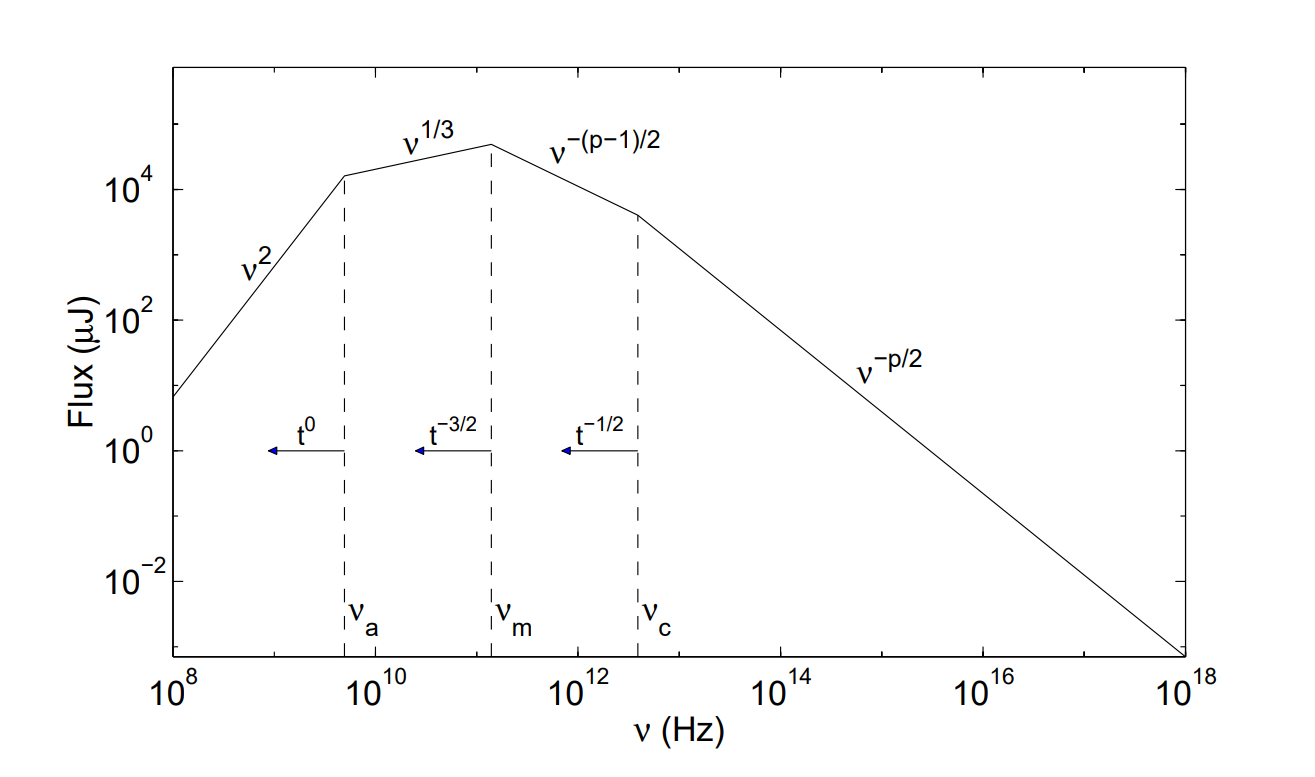
\includegraphics[width=0.8\linewidth]{sari_spectrum}
    \caption[Spectral energy distribution of a relativistic shock]{Spectrum of the relativistic shock in the canonical GRB afterglow model of \citet{2002ApJ...568..820G}. The spectrum consists of four segments with break frequencies $\nu_a$, $\nu_m$ and $\nu_c$ that evolve adiabatically and scale with time as denoted by the arrows. Figure modified from \citep{1998ApJ...497L..17S}.}
    \label{fig:sari_spectrum}
\end{figure}

The canonical GRB afterglow model of \citet{2002ApJ...568..820G} is based on the self-similar solution for the expansion of a relativistic blast wave with Lorentz factor $\gamma$, described by \citet{1976PhFl...19.1130B} with a variety of adjustments to account for radiative effects \citep{1997ApJ...489L..37S,1998ApJ...509..717C}. While this model explicitly describes a spherical blast wave, it is a valid approximation to the outflow of a jet as long as the lateral expansion of the jet remains negligible, i.e. $\gamma \gg \theta_j^{-1}$ \citep{1994AIPC..307..495P}. It is assumed that a fixed fraction, $\epsilon_B$, of the blast waves energy is deposited into the magnetic field, and that the energy of the electrons behind the shock follows a power-law distribution of the form $N(\gamma)\propto \gamma^{-p}$ above some Lorentz factor $\gamma > \gamma_m$. The fraction of the total energy deposited into the electrons is given by $\epsilon_e$.

The spectrum of the resulting emission is described by a series of 4 power-law segments as seen in Figure \ref{fig:sari_spectrum}. The location of the 3 break frequencies are given in terms of the isotropic equivalent energy (in units of $10^{52}$\,erg), $E_{52}$, the time post-merger (in days), $t_d$, the redshift of the merger, $z$, the energy density of the electrons, $e$, and the circum-merger density (in units of cm$^{-3}$), $n_0$,
\begin{align}
    \nu_a &= 1.24\times10^9 {\,\rm Hz} \left(\frac{p-1}{3p+2}\right)^{3/5}(1+z)^{-1}\bar{\epsilon_e}^{-1}\epsilon_B^{1/5} n_0^{3/5} E_{52}^{1/5}\\
%\end{equation}
%\begin{equation}
    \nu_m &= 3.73\times 10^{15} {\,\rm Hz} \left(\frac{p-0.67}{\sqrt{1+z}}\right) \bar{\epsilon_e}^{2} \epsilon_B^{1/2} E_{52}^{1/2} t_d^{-3/2}\\
%\end{equation}
%\begin{equation}
    \nu_c &= 6.37\times 10^{13} {\,\rm Hz} \left(\frac{p-0.46}{e^{1.16p}\sqrt{1+z}}\right) \epsilon_B^{-3/2} E_{52}^{-1/2} t_d^{-1/2}
\end{align}
where $\nu_a$ is the frequency below which synchrotron self-absorption is dominant, $\nu_m$ is the frequency corresponding to the synchrotron emission produced by electrons with minimum Lorentz factor $\gamma_m$, and $\nu_c$ is the synchrotron cooling frequency.

\citet{2014ARA&A..52...43B} estimates typical values are given by $\nu_a = 1\,$GHz, $\nu_m = 200t_d^{-1.5}$\,GHz and $\nu_c=200t_d^{-0.5}$\,PHz based on typical short GRB parameters of $E_{\rm iso} = 10^{51}$\,erg, $n=0.1$\,cm$^{-3}$ and $z=0.5$ and microphysics parameters of $\epsilon_e=0.1$, $\epsilon_B=0.01$, $p=2.4$. To compare expectations for afterglows associated with mergers detected by LIGO we also calculate typical break frequencies for $z=0.05$ \citep[corresponding to the LIGO horizon;][]{2018LRR....21....3A} with microphysics parameters $p=2.2$, $\epsilon_e=0.3$ $\epsilon_e=0.02$ based on typical values associated with known short GRBs \citep{2019ApJ...880L..23W}. This results in $\nu_a\sim 700\,$MHz, $\nu_m\sim 160t_d^{-1.5}$\,GHz and $\nu_c=240t_d^{-0.5}$\,PHz, suggesting that by $\sim 1$ month post-merger radio and X-ray observations will probe the same segment of the spectrum ($\nu_m<\nu<\nu_c$). This is in agreement with observations of GW170817 (see Section \ref{subsec:gw170817_afterglow_observations}).

If energy is continuously injected into the ejecta the lightcurve will rise, otherwise any observed increase is due to the evolution of the break frequencies. The decay of the lightcurve can then be used to characterise the geometry of the shock. In the spherical outflow regime the lightcurve will decay as $t^{-3(p-1)/4}$, while if the emission is jet-dominated it will decay as $t^{-p}$, assuming $\nu_m<\nu<\nu_c$ \citep{1999ApJ...519L..17S}.

\begin{figure}
    \centering
    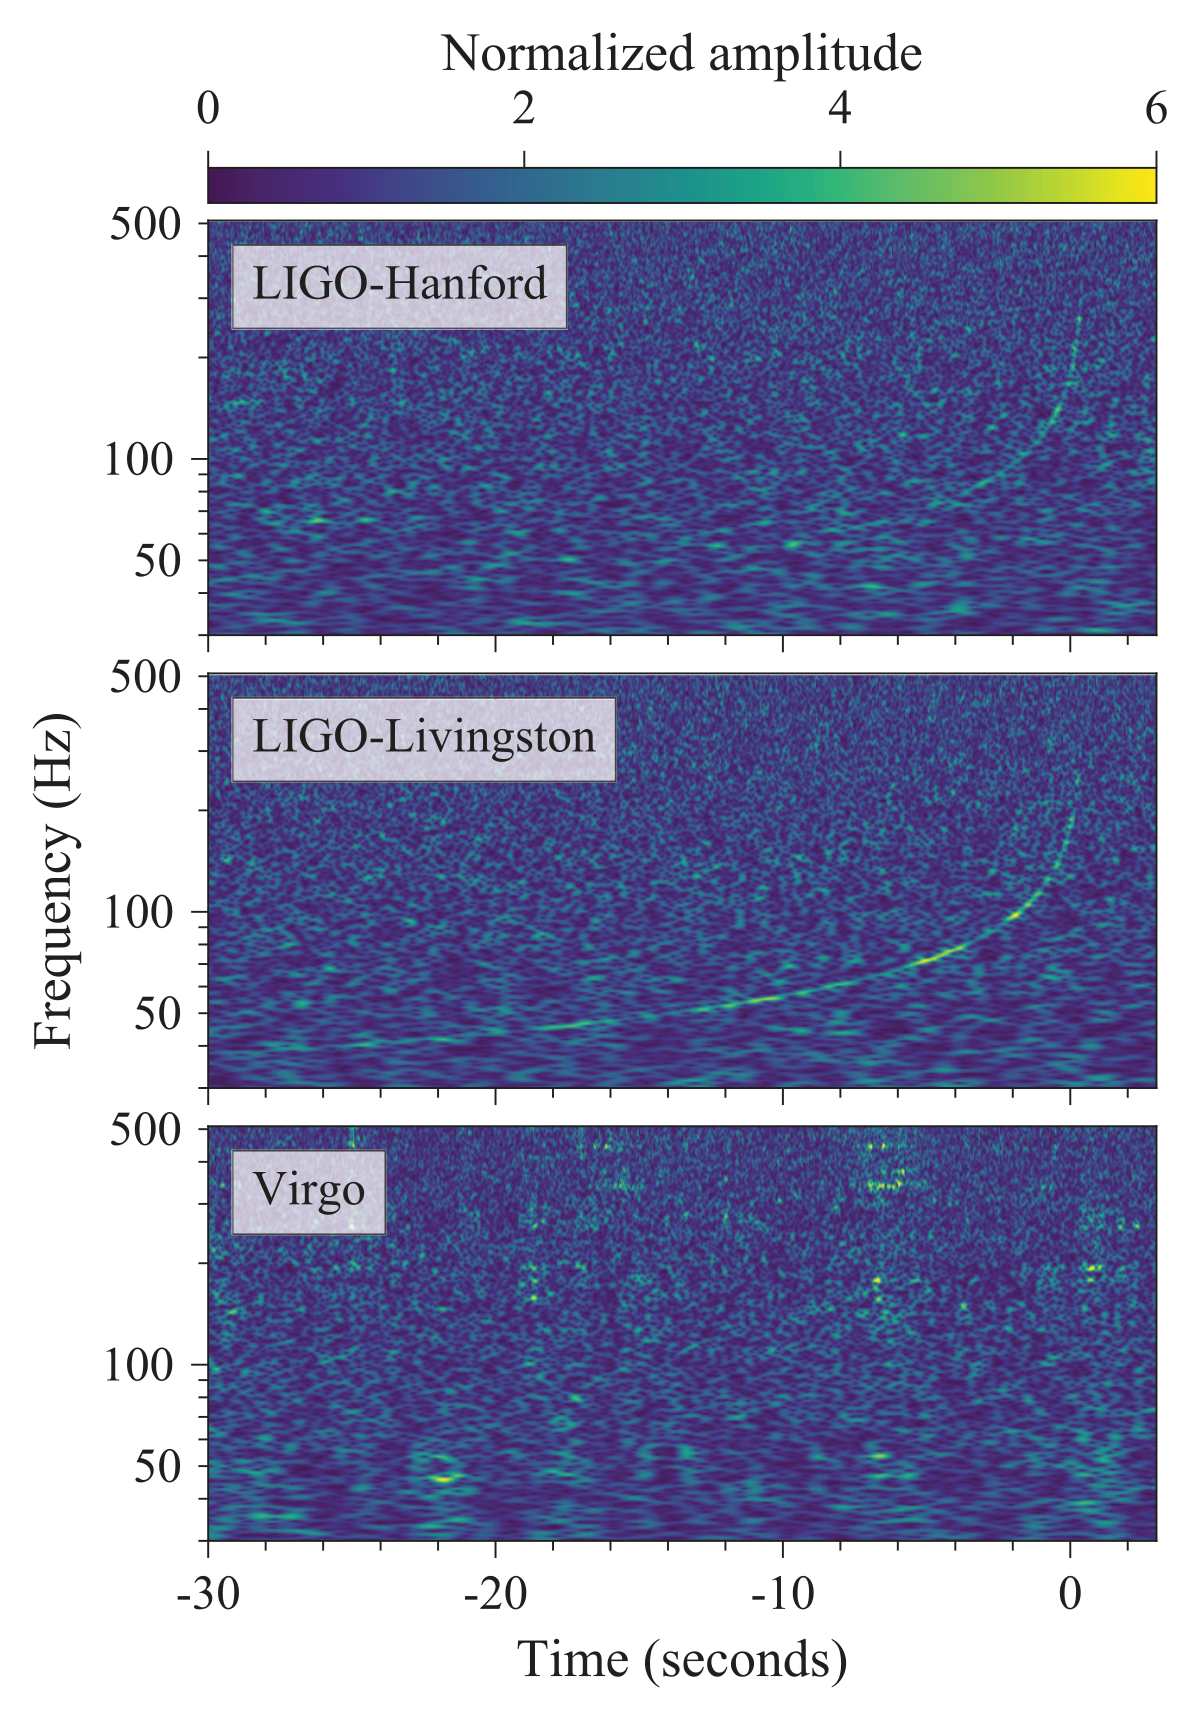
\includegraphics[width=0.7\linewidth]{GW170817_PSD}
    \caption[Gravitational Wave signal of GW170817]{Time-frequency representations of the gravitational wave signal produced by GW170817 as observed by the LIGO-Hanford (top), LIGO-Livingston (middle), and Virgo (bottom) detectors. Times are shown relative to August 17, 2017 12∶41:04
UTC. Figure reproduced from \citet{2017PhRvL.119p1101A}}
    \label{fig:GW170817_spectrogram}
\end{figure}

\pagebreak
\section{GW170817: The First Detection of a Neutron Star Merger}
\label{sec:gw170817_intro}
\subsection{Gravitational Waves and Gamma-rays}
\label{subsec:gw170817_gw_grb}
\citet{2017PhRvL.119p1101A} report the detection of a binary neutron star merger candidate on August 17, 2017 at 12:41:04 UTC in data from the LIGO Hanford detector with a signal-to-noise (SNR) ratio of 18.8. An offline analysis of data from the LIGO Livingston detector revealed the presence of an unrelated noise artefact 1.1\,s pre-merger, and after modelling and subtracting the artefact, the gravitational wave was clearly visible with an SNR of 26.4. While the Virgo detector was also operating at the time, it did not detect the signal due to its lower overall sensitivity and the antenna pattern relative to the location of the merger.

The merger was initially localised to 31$\,\deg^2$, before being refined to 28$\,\deg^2$ within days \citep{2017PhRvL.119p1101A}. A search of galaxy catalogues found 49 galaxies within the localisation \citep{2017Sci...358.1559K}, as seen in Figure \ref{fig:gw170817_localisation}. Further parameter estimates at later times improved the localisation to 16$\,\deg^2$ \citep{2019PhRvX...9a1001A}.

The Fermi Gamma-Ray Burst Monitor (GBM) detected a short GRB spatially coincident with the binary neutron star candidate 1.74\,s after to the merger \citep{2017ApJ...848L..14G,2017ApJ...848L..13A}. This burst was also detected at low significance \citep{2017ApJ...848L..15S} by the International Gamma-Ray Astrophysics Laboratory (INTEGRAL). The probability that the gravitational wave signal and GRB are unrelated was quantified by considering both events as independent Poisson processes and comparing the rate of both types of detection. The probability that the two events were temporally coincident but unrelated is $5\times 10^{-6}$. A comparison of the sky localisation of both detections showed that the probability of a chance spatial coincidence was 0.01, resulting in an overall probability that the events are unrelated of $5\times 10^{-8}$ \citep{2017ApJ...848L..13A}.

This joint detection of light and gravitational waves from the same source has a variety of implications for astrophysics and fundamental physics as a whole. The small difference in arrival time suggests that gravitational waves propagate at the speed of light to within a factor of $\sim 10^{15}$, although this precision may be underestimated by up to two orders of magnitude if the gravitational wave signal and GRB emission were asynchronous as many models predict \citep[e.g.][]{2017ApJ...850L..24G,2018ApJ...867...18N,2020ApJ...898...59L}. In turn, this rules out a multitude of theories regarding Dark Energy \citep{2017PhRvL.119y1304E} and gravity \citep{2018IJMPD..2747027S,2019PhRvL.123a1102A}. Most importantly this joint detection confirms the long-predicted connection between neutron star mergers and short GRBs \citep{1986ApJ...308L..43P,1989Natur.340..126E,1992ApJ...395L..83N}, although questions remain as to whether all neutron star mergers produce short GRBs and similarly, whether all short GRBs are produced by neutron star mergers.

\begin{figure}
    \centering
    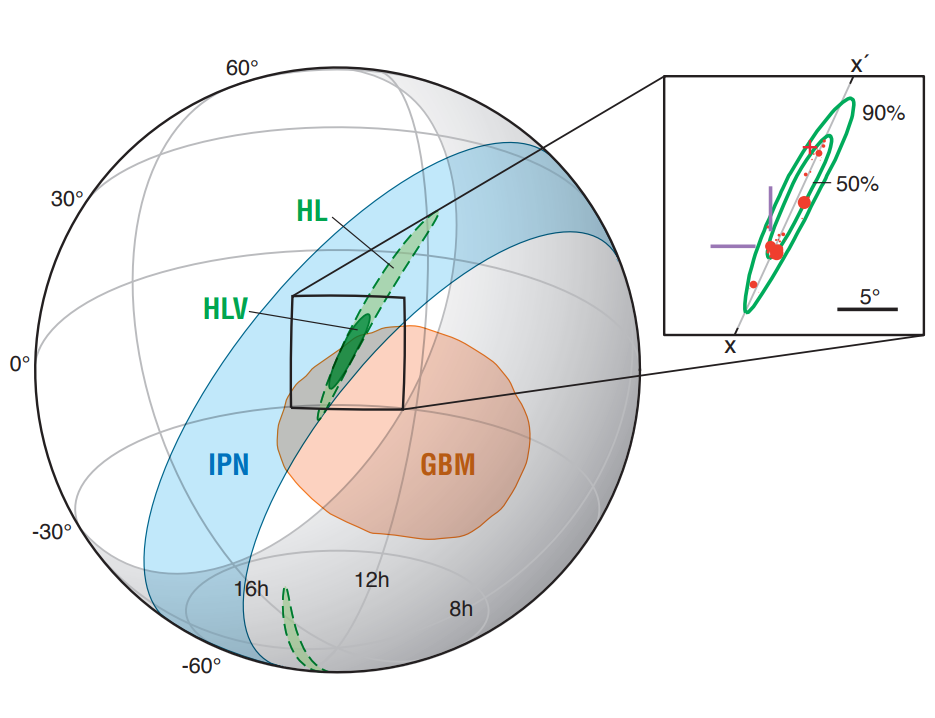
\includegraphics[width=0.8\linewidth]{Kasliwal_image}
    \caption[Localisation of GW170817]{Localisation of GW170817. The LIGO and full LIGO/Virgo localisations are shown in light and dark green respectively. The localisation from Fermi is shown in orange, and triangulation of the GRB using the Interplanetary Network (Fermi and INTEGRAL) is shown in blue. The inset shows the 50\% and 90\% contours with crosshairs marking the location of GW170817. Red markers show the 49 candidate host galaxies within the localisation volume, with marker size proportional to stellar mass. Figure adapted from \citet{2017Sci...358.1559K}.}
    \label{fig:gw170817_localisation}
\end{figure}

\subsection{Discovery of an Electromagnetic Counterpart}
Approximately 11 hours post-merger the detection of a candidate optical counterpart was announced by the One-Meter, Two-Hemisphere (1M2H) team \citep{2017Sci...358.1556C}, associated with NGC\,4993, one of the top-ranked host galaxy candidates. This counterpart was also independently detected by five other teams in observations carried out prior to the initial announcement \citep{2017Natur.551...64A,2017ApJ...850L...1L,2017ApJ...848L..16S,2017ApJ...848L..27T,2017ApJ...848L..24V}. Over the next few days comprehensive follow-up with ultraviolet, optical and infra-red (UVOIR) facilities was carried out, revealing a rapid dimming of the initially blue emission, and a brightening of redder emission. Spectroscopy of the source showed no significant emission or absorption lines, something rarely observed in the thousands of optical transients that have been detected. The rapidly peaking blue emission followed by a slower rising red component, along with the featureless spectra, was consistent with models for a kilonova produced by a neutron star merger \citep{2015NatPh..11.1042H,2015MNRAS.450.1777K,2015MNRAS.446.1115M,2016ApJ...829..110B}. Late-time high-resolution spectroscopy found the signatures of elements produced by r-process nucleosynthesis, thereby confirming the nature of the optical emission \citep{2017ApJ...848L..19C,2017Sci...358.1559K,2017Natur.551...67P}. This discovery simultaneously confirmed previous predictions that neutron star mergers are the origin of many of the heavy elements in Universe \citep{1974ApJ...192L.145L,1982ApL....22..143S,1999ApJ...516..381F}.

While deep observations with a variety of X-ray telescopes began almost immediately after the discovery of the optical counterpart, it was not until 9 days post-merger that X-ray emission was detected \citep{2017Natur.551...71T}. This detection was confirmed in a second epoch of observations 15 days post-merger \citep{2017ApJ...848L..25H,2017Natur.551...71T}, just prior to the location of GW170817 being unobservable with leading X-ray facilities due to solar proximity.

Two independent observations with the Karl G. Jansky Very Large Array (VLA) 16 days post-merger claimed a low-significance detection of radio emission consistent with the coordinates of the merger, which was confirmed by an observation with the Australia Telescope Compact Array (ATCA) two days later \citep{2017Sci...358.1579H}. Further observations in the following weeks showed that the radio emission had continued to rise \citep{2017ApJ...848L..21A,2017Sci...358.1579H}. We discuss the evolution of the radio lightcurve and it's implications in Section \ref{subsec:gw170817_afterglow_observations}.

A full description of the discovery of the electromagnetic counterpart and the initial follow-up can be found in \citet{2017ApJ...848L..12A} and references therein.

% \begin{figure}
%     \centering
%     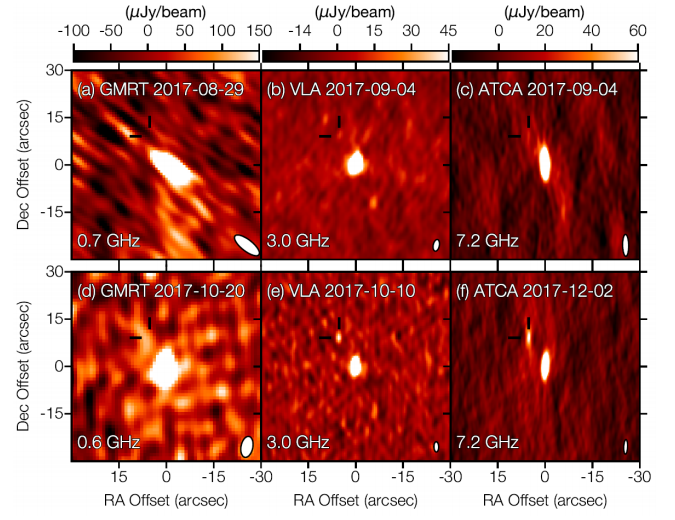
\includegraphics{GW170817_radio_imaging}
%     \caption[Radio imaging of GW170817]{PLACEHOLDER IMAGE: Will replace with a series of ATCA images in a similar format}
%     \label{fig:gw170817_radio_imaging}
% \end{figure}

\begin{figure}
    \centering
    \animategraphics[controls]{1.2}{gw170817_animation_frames/}{1}{12}
    \caption[ATCA imaging of GW170817]{ATCA imaging of GW170817 up to one year post-merger. The position of the merger is denoted by white crosshairs, and the central radio source is host galaxy emission. Please use Adobe Acrobat to view the animated graphic.}
    \label{fig:gw170817_radio_imaging}
\end{figure}

\pagebreak
\subsection{Observations of the Radio Afterglow}
\label{subsec:gw170817_afterglow_observations}
Continued radio observations with the ATCA, VLA and Giant Metrewave Radio Telescope (GMRT) showed that the radio emission rose according to a spectral and temporal power law, $S_\nu(t) \propto \nu^{-0.6} t^{0.8}$ \citep{2018Natur.554..207M}. These observations suggested the emission was not produced by a standard relativistic jet viewed off-axis, but instead originated from a mildly-relativistic, quasi-spherical outflow.

In December 2017 the Chandra X-ray telescope emerged from sun-block and was able to continue observations. Contemporaneous X-ray, optical and radio observations showed that the spectrum was well-fit by a single power law, suggesting that the synchrotron cooling break, $\nu_c$, had not yet transitioned into the X-ray band \citep{2018MNRAS.478L..18T,2018ApJ...856L..18M}. The long spectral baseline of these observations also refined estimates of the spectral index to $\alpha=0.58$ and constrained the index of the electron energy distribution to $p=2.17\pm 0.01$ \citep{2018ApJ...856L..18M}.

The next breakthrough came from radio observations carried out as part of this thesis, which provided strong evidence that the non-thermal lightcurve had peaked at approximately 150 days post-merger and had begun to decline \citep{2018ApJ...858L..15D}. Chapter \ref{chap:gw170817_turnover} details this discovery and it's implications for afterglow modelling.

Multiple works detail the gradual refinement of merger parameters based on continued monitoring \citep{2018ApJ...863L..18A,2018ApJ...868L..11M,2019MNRAS.483.1912P}. However, the similarities in the lightcurves predicted by competing models for the outflow geometry necessitate some other form of measurement to distinguish between them \citep{2018MNRAS.478..407N}. \citet{1999ApJ...524L..43S} showed that the relativistic jet associated with GRBs should produce linearly polarised radio emission, and that the emission centroid should also exhibit proper motion. Both the polarisation fraction and the amplitude of proper motion should be maximum at the time of the lightcurve peak. 

Observations between 75 and 230 days post-merger with the Very Long Baseline Array (VLBA) suggested that the centroid of the radio emission had shifted significantly \citep{2018Natur.561..355M}. The apparent velocity of this shift was calculated to be $\beta_{\rm app} = 4.1$, measured in terms of the speed of light, $c$. These findings were later confirmed with an independent observation using global VLBI from 207 days post-merger \citep{2019Sci...363..968G}. The observation of this motion suggests that the observed late-time emission originated from the jet, and enables a direct measurement of the associated Lorentz factor ($\Gamma=\beta_{\rm app}$).

\citet{2018ApJ...861L..10C} carried out a deep search for linear polarisation and constrained the polarisation fraction to $<12$\% at 244\,days post-merger. This result suggests that a significant component of the magnetic field of the jet is oriented perpendicular to the shock front. Specifically, the models of \citet{2018MNRAS.478.4128G} suggest $b=\langle B^2_{\rm sn}\rangle/\langle B^2_{\rm sp}\rangle \gtrsim 0.75$, where $B_{\rm sn}$ and $B_{\rm sp}$ are the components of the magnetic field in the direction of the shock normal and in the plane of the shock respectively. More recent modelling suggests $0.66 < b < 1.49$ \citep{2020MNRAS.491.5815G}.

By $\sim 750$\,days post-merger the radio afterglow had faded beyond detection, with an observation with the VLA at $\Delta T=767\,$d finding only marginal evidence for continued emission \citep{2020arXiv200602382M} and an ATCA observation at $\Delta T=990\,$d finding no emission at 2.1\,GHz \citep{2020arXiv200601150T}. However, the X-ray emission remains detectable at $\Delta T=940\,$d (the latest observation at the time of writing) although it continues to rapidly fade consistent with the afterglow of a jet \citep{2020arXiv200601150T,2020RNAAS...4...68H}. These late-time X-ray observations appear to marginally deviate from the simple power-law decline, perhaps suggesting more complex temporal evolution or the emergence of emission from the dynamical ejecta. However, this deviation is within observational uncertainties and continued monitoring is necessary to determine whether it is statistically significant.

\begin{figure}
    \centering
    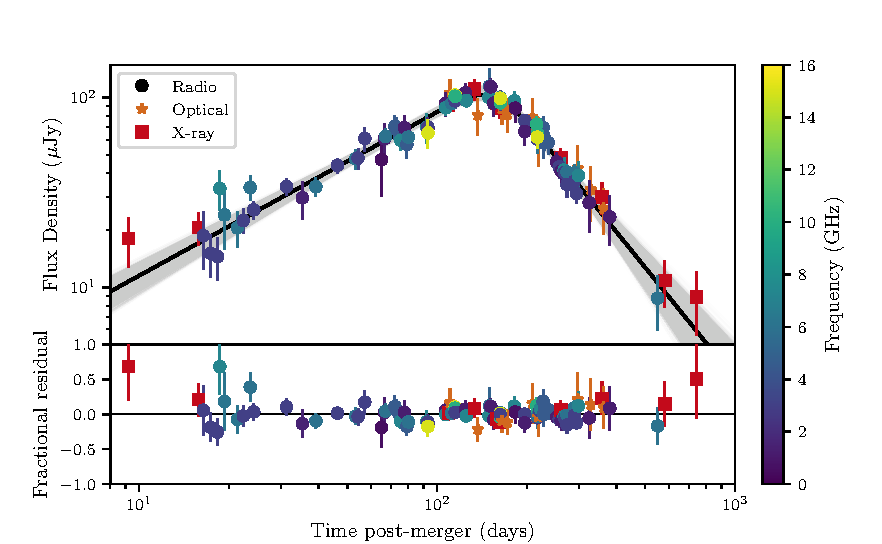
\includegraphics{GW170817_nonthermal_thesis}
    \caption[Lightcurve of non-thermal emission from GW170817]{Detections of non-thermal emission from GW170817 with radio (circles), optical (stars) and X-ray (squares) facilities compiled by \citep{2020arXiv200602382M}. The lightcurve has been scaled to 7.25\,GHz, corresponding to the central frequency of our ATCA observations, based on a spectral index of $\alpha=-0.585$, while the original observing frequency is denoted by the colourbar. A smoothed broken power law has been fit to the data, with fractional residuals shown in the bottom panel.}
    \label{fig:gw170817_nonthermal_lightcurve}
\end{figure}

\subsection{Modelling the Non-thermal Afterglow}
\label{subsec:GW170817_afterglow_models}
The exact geometry of the merger, and the origins of the observed emission, were a source of strong contention for some time. While it was generally agreed that the `top-hat' jet structure \citep{1965PhFl....8.1428G} commonly used to describe previous short GRB afterglows was inconsistent with the slow rise of the radio afterglow \citep{2017Sci...358.1559K,2018ApJ...856L..18M}, there was little agreement as to the outflows true nature. A wide range of models have been proposed, but they generally fall into one of two categories, with the emission being produced by either a quasi-spherical outflow or an off-axis jet.

A quasi-spherical outflow could be produced in a variety of ways. \citet{2018MNRAS.474L...7S} suggest that the merger may not have launched a jet at all. Instead, the final stages of the merger may have resulted in the formation of a turbulent magnetic dynamo, which dissipates via magnetic reconnection, thereby accelerating electrons to relativistic speeds and launching a `fireball' \citep{2013ApJ...769L..29Z,2015ApJ...809...39G}. While the early rise of the lightcurve is inconsistent with emission from the dynamical ejecta scenario proposed by \citet{2011Natur.478...82N}, a small fraction of the ejecta would be accelerated to mildly relativistic speeds. This `fast tail' is sufficient to enhance the the radiation produced by the interaction between the outflow and the circum-merger medium  and produce the observed emission \citep{2018ApJ...867...95H}. However, this scenario is inconsistent with the rapid peak and decline of the observed lightcurve and can now be ruled out.

Even if a jet is initially launched by the merger, it may not break out of the surrounding ejecta (comparable to a standard short GRB) and instead be choked, producing an energetic cocoon \citep{2017ApJ...834...28N,2018MNRAS.479..588G,2018MNRAS.473..576G}. While there is a variety of jet types, all will produce a cocoon, regardless of whether or not they successfully break out \citep{2018MNRAS.478..407N}. The vast majority of jet models that aim to explain the emission from GW170817 are `structured jets' - i.e. an axisymmetric relativistic outflow with some angular or radial dependence. Some assume that the jet has a particular angular structure, such as power-law or Gaussian profiles \citep[e.g.][]{2019NatAs...3..940H,2020arXiv200601150T,2020MNRAS.495.3780N}, while others are more physically motivated \citep[e.g.][]{2018MNRAS.473L.121K,2018ApJ...863...58X} or motivated by the observed lightcurve alone \citep{2020arXiv200713116T}. However, \citet{2020arXiv200501754N} note that the majority of these fits ignore the observed centroid motion and consider only the lightcurve, which cannot uniquely determine the inclination angle, $\theta_{\rm obs}$. The result is large uncertainties in the value of $\theta_{\rm obs}$ inferred by each model, and inconsistencies between models.

The observed centroid motion indicates that the radio emission originates from some form of (at least) mildly relativistic ejecta, but at the time of writing there is no clear evidence to preference one particular model or geometry over another. While the leading models discussed above are all objectively different, they predict qualitatively similar lightcurves that are indistinguishable with the observational data at hand. With the benefit of hindsight, higher cadence monitoring between 10 and 100 days may have been able to determine the presence more complex temporal evolution predicted by some models \citep[e.g.][]{2018PhRvL.120x1103L,2020arXiv200602382M}. However, this measurement would still likely have been limited by the sensitivity of the observations. Similarly, observations thousands of days post-merger could in principle reveal a flattening decline predicted by other models \citep{2020arXiv200601150T}, but are impossible due to the limited sensitivity of X-ray and radio facilities. While population studies of future events may reveal the standard mechanisms behind non-thermal emission from neutron star mergers, it is likely that the precise structure of the jet launched by GW170817 in particular will forever elude us.

\pagebreak
\section{Thesis Goals}
\label{sec:thesis_goals}
The 2015 discovery of gravitational waves from a binary black hole merger provided a new avenue for astronomers to probe the Universe. The fields of gravitational waves and multi-messenger astronomy have evolved rapidly since then, with the detection of gravitational waves and light from a neutron star merger 2 years later, and a veritable menagerie of compact object coalescences detected in 2019-20. Planned upgrades to existing gravitational wave detectors, and proposed future detectors, will enable the detection of more mergers at even larger distances, and with improved localisations that will be conducive to follow-up with electromagnetic facilities. Simultaneously, radio astronomy is undergoing a revolution as we move towards the era of the Square Kilometre Array (SKA). SKA precursors like the Australian Square Kilometre Array Pathfinder (ASKAP) and MeerKAT are finally achieving design sensitivity and are beginning to carry out unprecedented surveys of the sky. These next-generation telescopes will enable astronomers to undertake most sensitive surveys for radio transients to-date, including searches for radio counterparts to gravitational wave events.

The work in this thesis spans a critical period in the development of the fields of multi-messenger and radio-transient astronomy. It begins with the detection of the first neutron star merger, GW170817, where I played a significant role in the detection of radio emission and the long-term monitoring of its evolution. I developed an algorithm to optimise follow-up observations with ASKAP, and then carried out ASKAP follow-up of the first neutron star-black hole merger, GW190814. This thesis also comprehensively outlines future prospects for the field and quantifies expectations for future detections of radio counterparts, the use of VLBI observations to directly measure outflow structure and how high-cadence radio monitoring can be used to constrain the size of outflows.

In Chapter \ref{chap:gw170817_turnover} I demonstrate evidence for a turnover in the radio lightcurve of GW170817 based on observations with the ATCA and VLA

In Chapter \ref{chap:optimised_followup} I outline the capabilities of ASKAP in performing follow-up of gravitational wave events, and describe an optimised observing strategy to do so.

Chapter \ref{chap:GW190814} applies the results of the previous chapter to follow-up of GW190814, where I undertook the most sensitive widefield search for radio transients to-date, and placed constraints the merger properties.

In Chapter \ref{chap:neutron_star_merger_outflows} I discuss prospects for constraining the geometry of merger outflows using Very Long Baseline Interferometry to detect relativistic expansion and motion of the outflow and high-cadence monitoring of scintillation to infer source size.

Chapter \ref{chap:radio_gw_detectability} outlines the various contributions radio observations can make to the gravitational wave follow-up effort and quantifies prospects for detecting afterglows with existing and planned facilities.

To conclude, Chapter \ref{chap:conclusion} summarises the work of this thesis and places it in the broader context of multi-messenger astronomy.


